\documentclass[12pt,a4paper]{article}
\usepackage[UTF8]{ctex}
\usepackage{amsmath, amssymb}
\usepackage{geometry}
\usepackage{booktabs}
\usepackage{graphicx}
\usepackage{float}
\geometry{left=2.5cm, right=2.5cm, top=2.5cm, bottom=2.5cm}
\title{\textbf{问题四 灵敏度分析报告}\\[4pt]
\large VLSI 布图规划设计 --- 模型参数灵敏度分析}
\author{2026 年第七届"华数杯"大学生数学建模竞赛 B 题}
\date{2026/08}
\begin{document}
\maketitle

问题 4 为穷举确定性求解，无随机参数；灵敏度分析考察\textbf{模型输入
变化}对最优解的影响，验证最优解（24）的稳定性与凹角支撑解码的必要性。

\section{S1：旋转自由度消融}

将允许的旋转集合从四向逐步收紧为 0°/90° 与仅 0°，观察最小包围盒面积
的变化，检验四向旋转的贡献。

\begin{figure}[H]
\centering
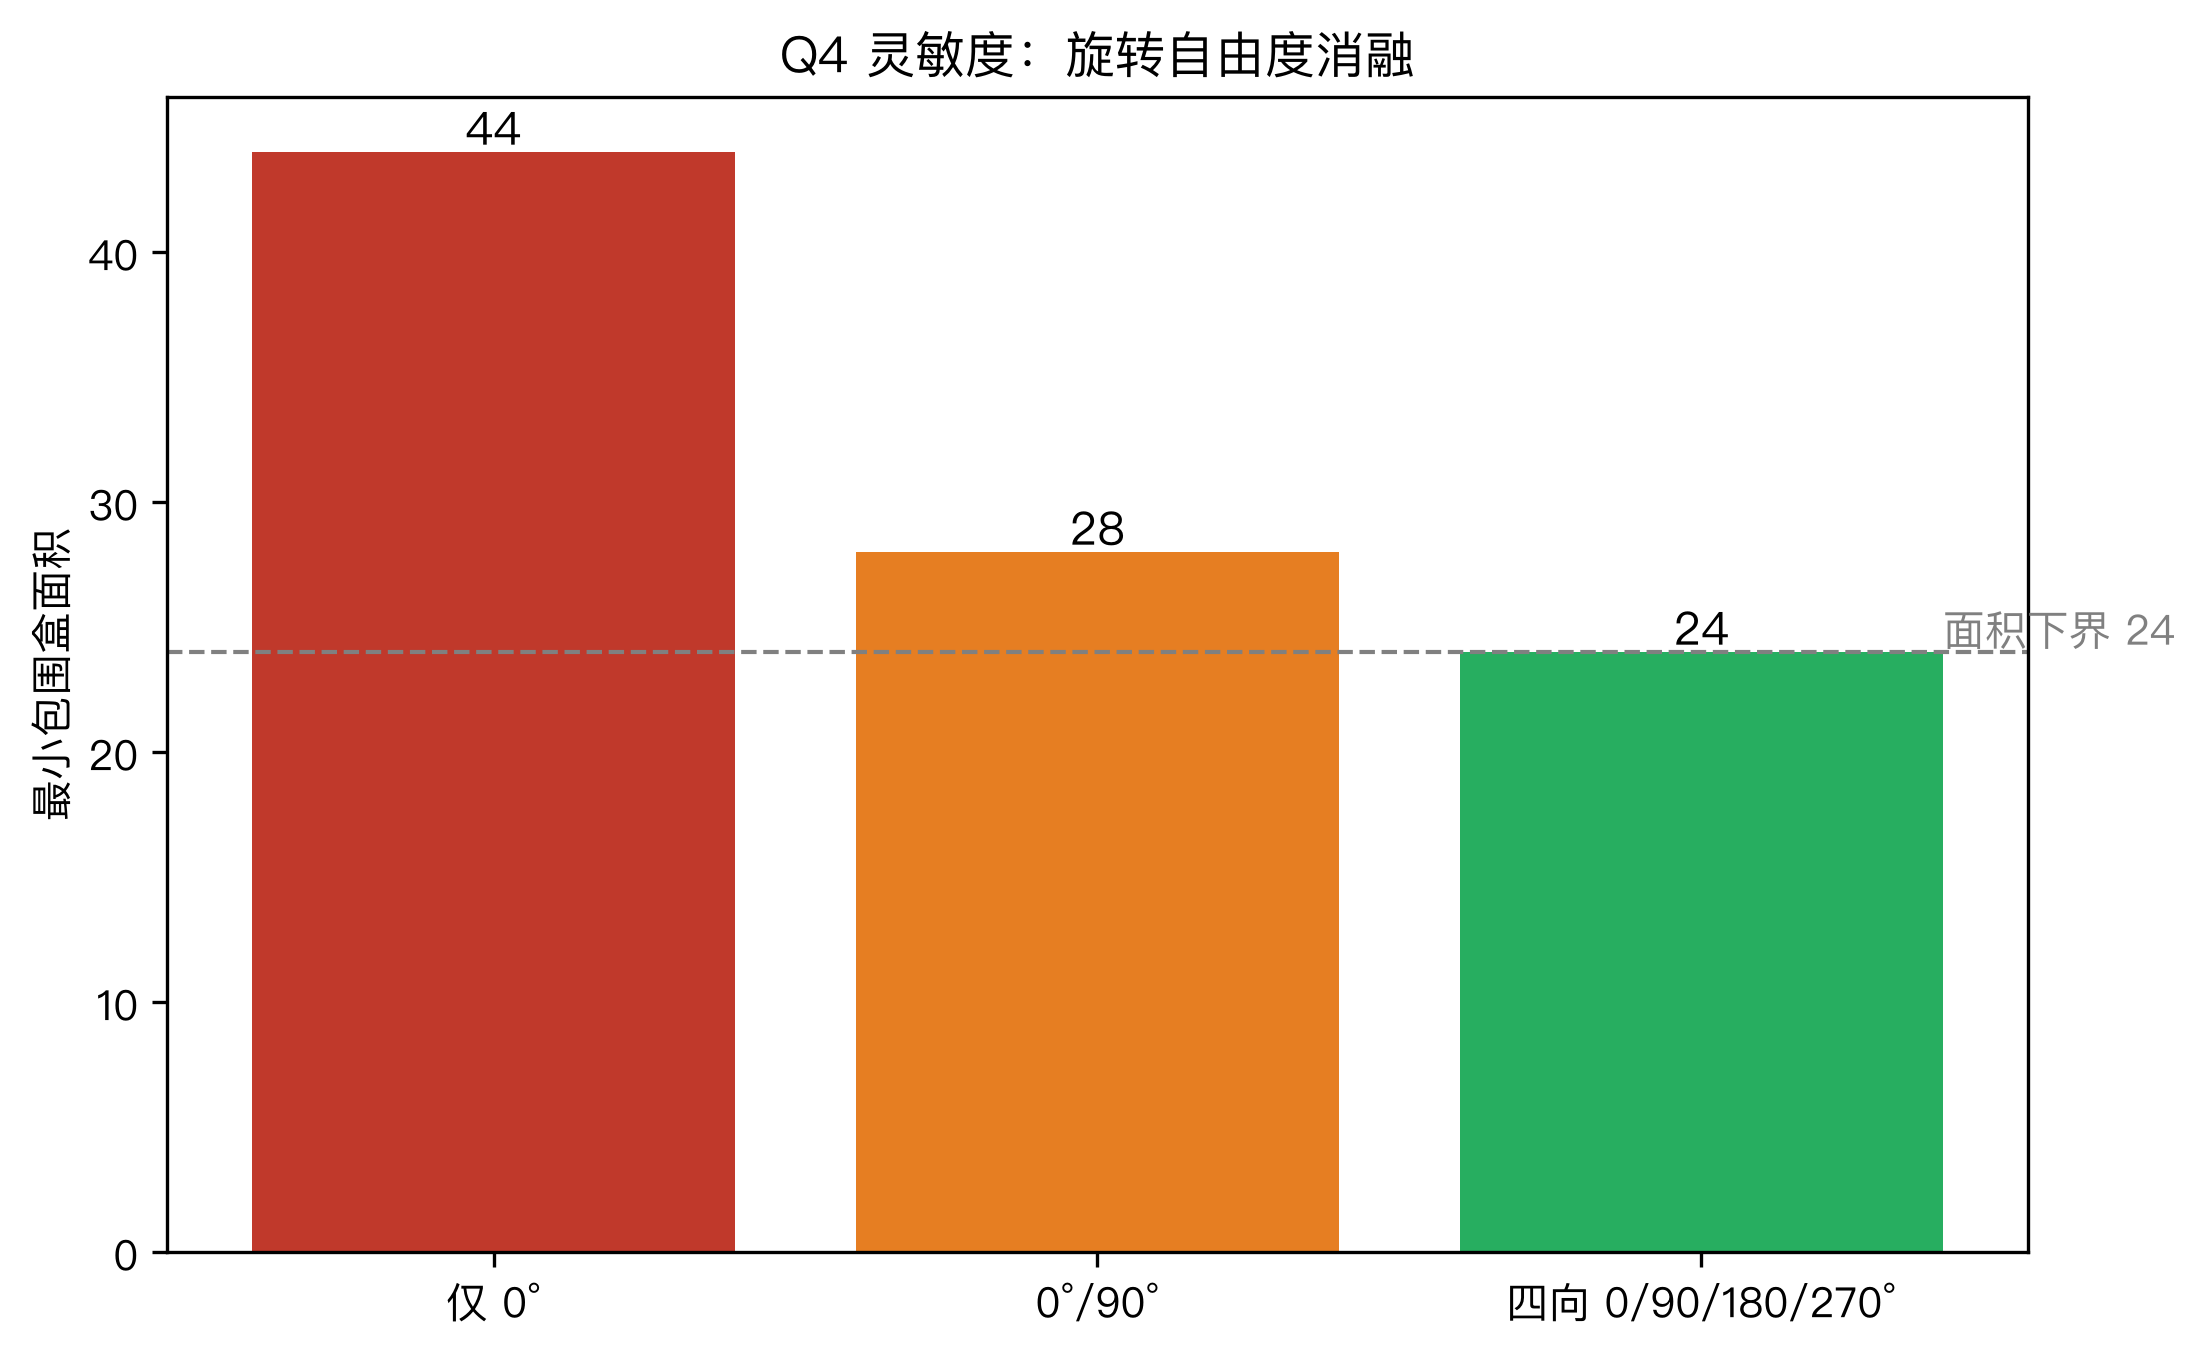
\includegraphics[width=0.82\textwidth]{q4_rotation_freedom_ablation.png}
\caption{旋转自由度消融}
\end{figure}

  \begin{table}[H]
  \centering
  \caption{S1 数据}\label{tab:q4s1}
  \begin{tabular}{lllll}
  \toprule
  rotation\_freedom & best\_area & bbox\_version\_area & valid\_layouts & total \\
  \midrule
  仅 0° & 44 & 52 & 336 & 336 \\
  0°/90° & 28 & 32 & 5376 & 5376 \\
  四向 0/90/180/270° & 24 & 32 & 86016 & 86016 \\
  \bottomrule
  \end{tabular}
  \end{table}

\textbf{结论}：仅 0° 旋转时最小面积 44，放宽到 0°/90° 降至 28，
四向旋转达到 24（面积下界）。旋转自由度对结果\textbf{有实质影响}
（24 vs 44，省 45\%）；最优解 24 需要四向旋转与凹角支撑共同作用。
所有消融配置均通过矩形级重叠检查。

\section{S2：模块尺寸扰动}

逐一将每个模块的分解矩形 $w, h$ 各 +1（面积增大），其余模块不变，
观察最优面积变化——检验最优解对尺寸扰动的敏感性。

\begin{figure}[H]
\centering
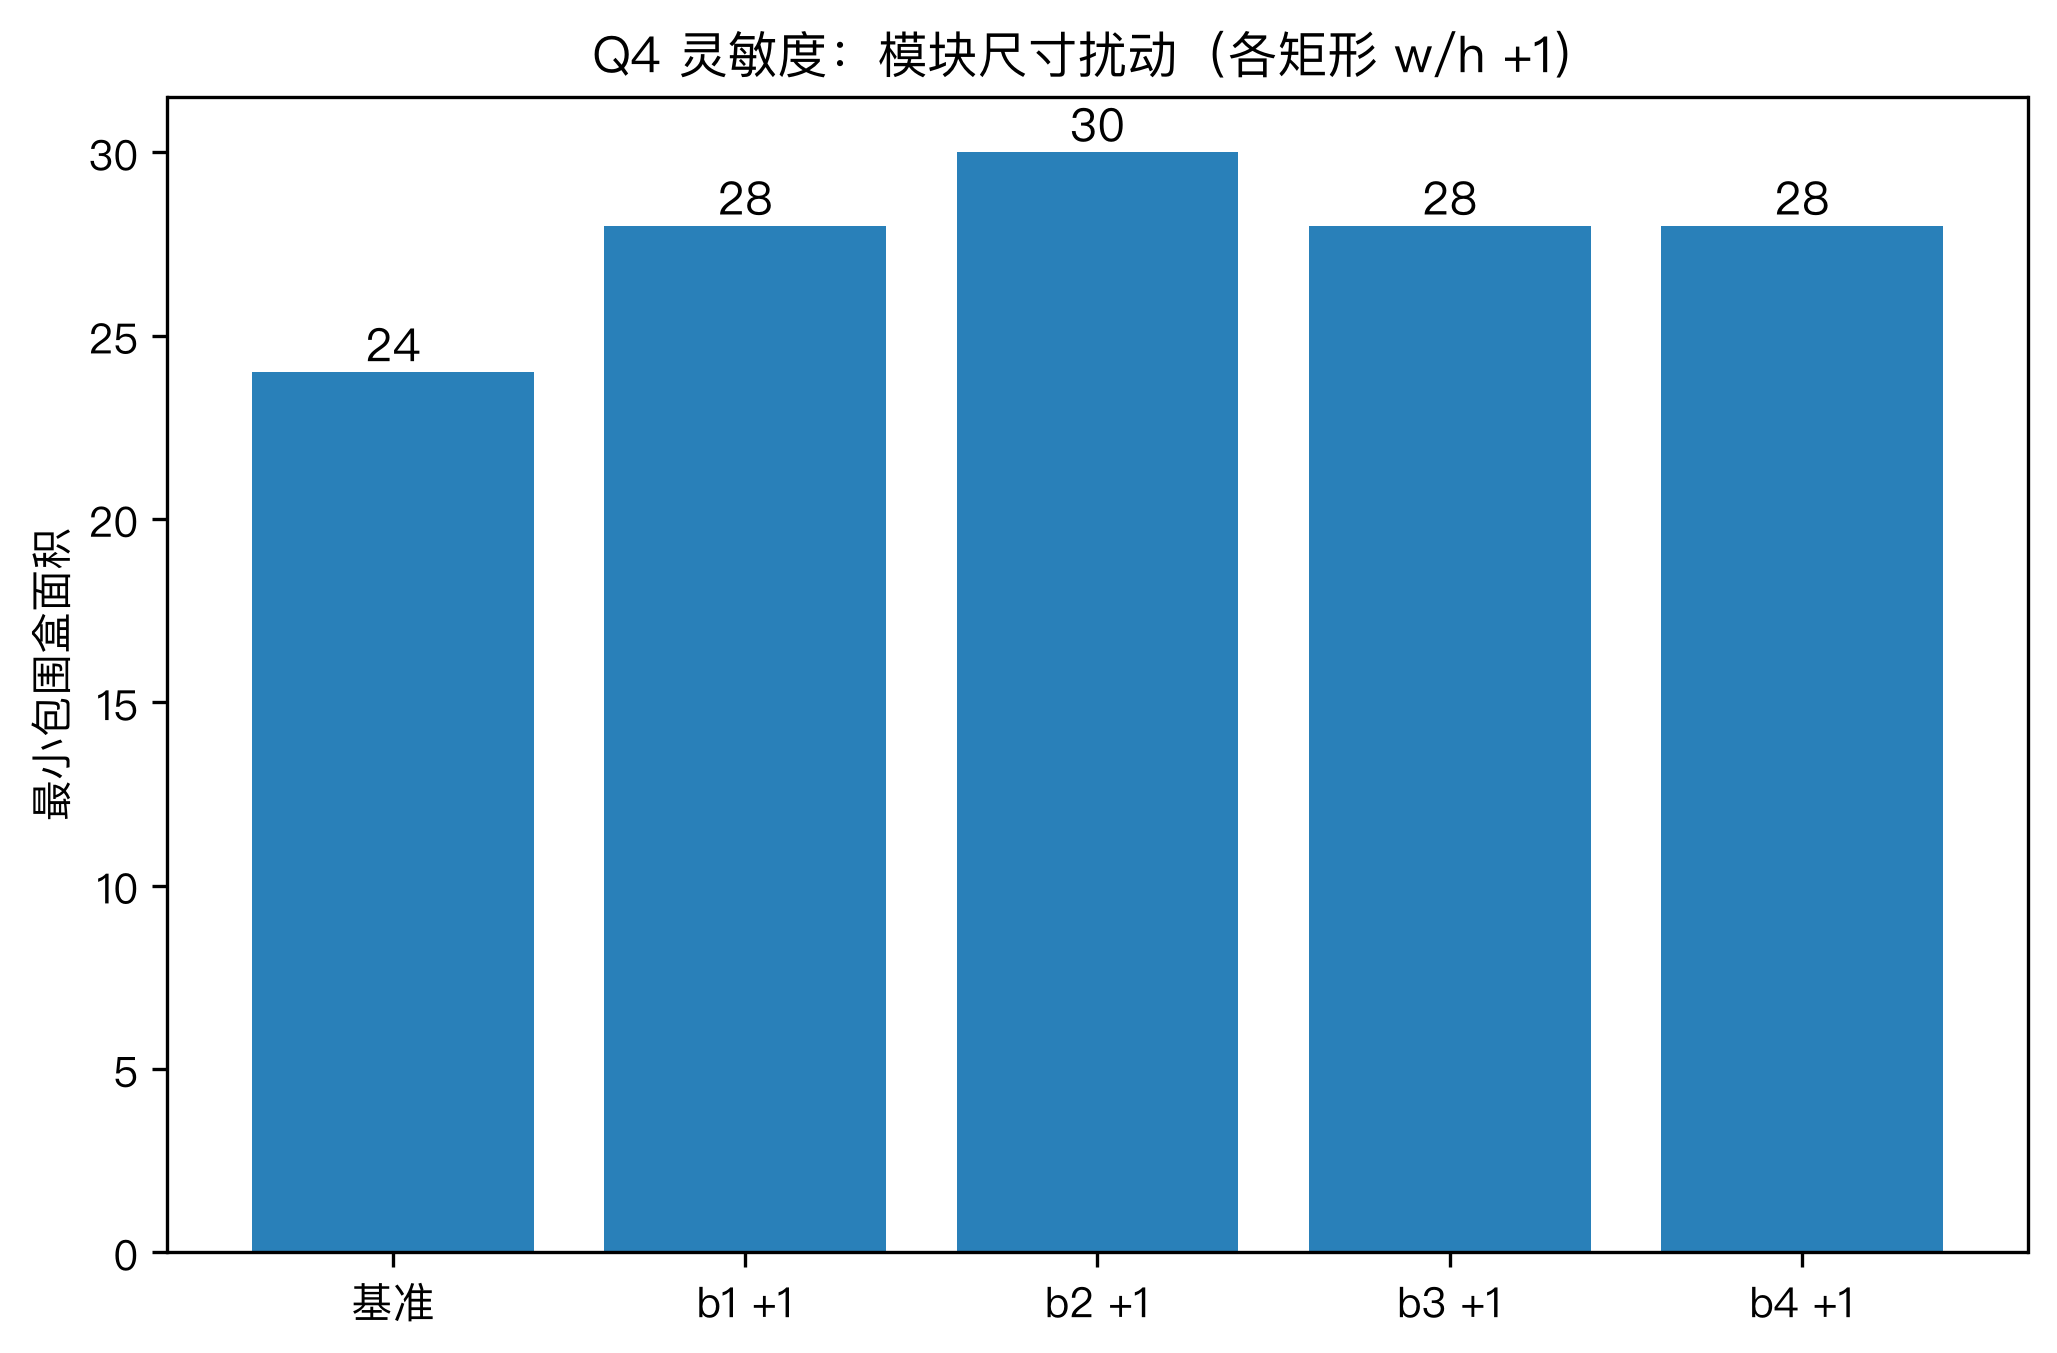
\includegraphics[width=0.82\textwidth]{q4_size_perturbation.png}
\caption{模块尺寸扰动后的最小面积}
\end{figure}

  \begin{table}[H]
  \centering
  \caption{S2 数据}\label{tab:q4s2}
  \begin{tabular}{llll}
  \toprule
  module & module\_area & best\_area & bbox\_version\_area \\
  \midrule
  基准 & 24 & 24 & 32 \\
  b1 +1 & 14 & 28 & 36 \\
  b2 +1 & 7 & 30 & 40 \\
  b3 +1 & 3 & 28 & 32 \\
  b4 +1 & 8 & 28 & 36 \\
  \bottomrule
  \end{tabular}
  \end{table}

\textbf{结论}：尺寸扰动后最优面积上升且\textbf{不再全部达到下界}——
b4（$1\times4\to1\times5$）仍达新下界 28，其余模块扰动后超过下界
2$\sim$5——说明 24 的完美铺满（零死区）对尺寸组合\textbf{敏感}，
是特定尺寸的巧合而非普遍性质。但所有扰动实例中\textbf{凹角精确支撑版
均显著优于 bbox 放置版}（28$\sim$30 vs 32$\sim$40），证明凹角支撑
解码的紧凑性优势对尺寸变化稳健。

\end{document}
